\documentclass[a4paper,11pt]{article}
\usepackage[utf8]{inputenc}
\usepackage{graphicx}
\usepackage{enumerate}
\usepackage{geometry}
\usepackage{fancyhdr}
\usepackage{minted}
\usepackage{xcolor}
\usepackage{listings}
\usepackage[colorlinks = true,
            linkcolor = blue,
            urlcolor  = blue,
            citecolor = blue]{hyperref}

\geometry{total={210mm,297mm},
left=25mm,right=25mm,%
bindingoffset=0mm, top=20mm,bottom=20mm}

\graphicspath{ {./images/} }
\renewcommand{\thesubsubsection}{\thesubsection.\alph{subsubsection}}
\renewcommand*\sfdefault{phv}
\renewcommand\familydefault{\sfdefault}

% \renewcommand{\thesubsubsection}{\thesubsection.\alph{subsubsection}}

% \newmintedfile{html}{
%     linenos,
%     breaklines,
%     python3,
%     numbersep=8pt,
%     frame=single,
%     framesep=3mm} 

\newcommand*{\TitleFont}{%
      \usefont{\encodingdefault}{\rmdefault}{b}{n}%
      \fontsize{16}{20}%
      \selectfont}

\linespread{1.3}

% my own titles
\makeatletter
\renewcommand{\maketitle}{
\begin{center}
\vspace{2ex}
{\huge \textsc{\TitleFont \@title}}
\vspace{1ex}
\\
\rule{\linewidth}{0.5pt}\\
\@author \hfill \@date
\vspace{4ex}
\end{center}
}
\makeatother

\definecolor{bg}{rgb}{0.95,0.95,0.95}


% custom footers and headers
\pagestyle{fancy}
\lhead{}
\chead{}
\rhead{}
\lfoot{title}
% \lfoot{\@title}
\cfoot{}
\rfoot{Page \thepage}
\renewcommand{\headrulewidth}{0pt}
\renewcommand{\footrulewidth}{0pt}
%%----------%%%----------%%%----------%%%----------%%%

\begin{document}

\newminted{python}{fontsize=\scriptsize, 
    linenos,
    python3,
    numbersep=8pt,
    frame=single,
    bgcolor=bg,
    framesep=3mm} 
\newminted{bash}{fontsize=\scriptsize, 
    linenos,
    numbersep=8pt,
    frame=single,
    bgcolor=bg,
    framesep=3mm} 



% \newminted{all}{linenos, frame=single}

% \usemintedstyle{monokai}
\usemintedstyle{manni}
% \usemintedstyle{xcode}
% \usemintedstyle{vs}
% \usemintedstyle{autumn}
% \usemintedstyle{colorful}
% \usemintedstyle{trac}


\title{Wi-Fi based access control system}

\author{Ali Abdulmadzhidov, Oleg Ilin, Emil Sharifulllin}

\date{\today}

\maketitle
\tableofcontents

\section{Introduction}
Wi-Fi is a technology that widespread and every year are manufactured millions of devices that contains Wi-Fi module. Inside the building turned on Wi-Fi on smartphone can be useful to be track using wireless sniffers. In our work we tried to investigate methods that allows us to detect violations of the restricted area based on active Wi-Fi device.

\section{Wi-Fi widespread}
Smart phones have become an important part of our daily lives due to their capabilities of accessing the web using WiFi and mobile data networks. Wi-Fi Alliance announced today that Wi-Fi shipments have reached 12 billion units, and are expected to surpass 15 billion units by the end of 2016. With an installed base of more than 6.8 billion devices, Wi-Fi has become one of the most prolific technologies around the world. Figure \ref{fig:chart} shows that in selected countries mean number of Wi-Fi devices per person is more than one. Modern Wi-Fi working principles allows us to implement additional solution for access control system.

\begin{figure}[h]
    \centering
    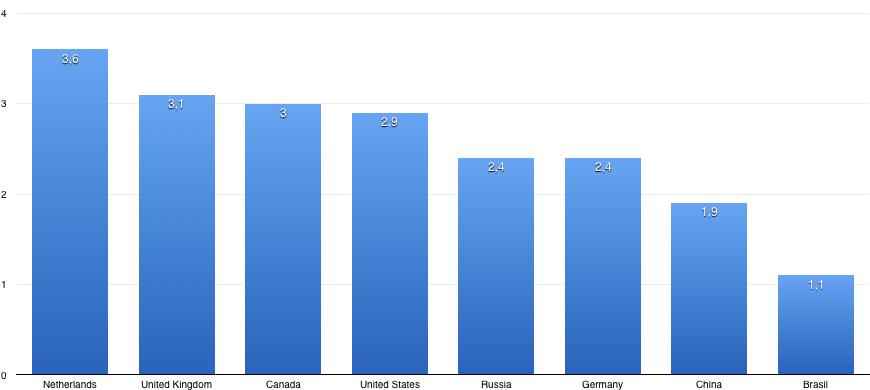
\includegraphics[width=0.8\textwidth]{chart}
    \caption{Average number of connected devices used per person in selected countries in 2014}
    \label{fig:chart}
\end{figure}
% \begin{center}
% 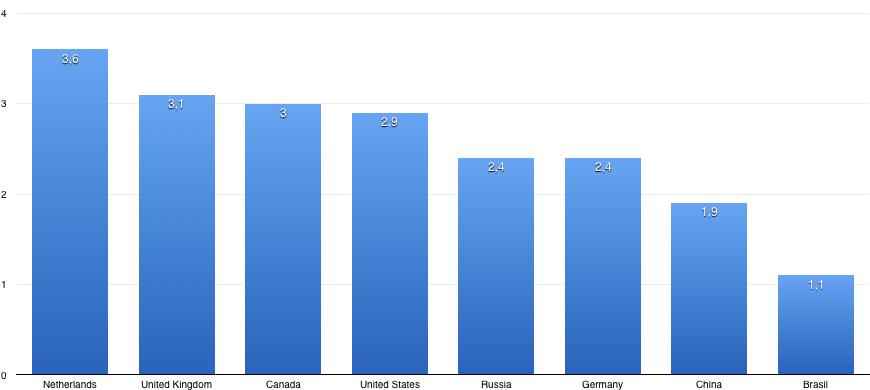
\includegraphics[width=15cm]{chart}
% \end{center}

\section{Wi-Fi basics}
Wi-Fi is a technology for wireless local area networking with devices based on the IEEE 802.11 standards. Wi-Fi most commonly uses the 2.4 gigahertz (12 cm) UHF and 5 gigahertz (6 cm) SHF ISM radio bands. Having no physical connections, it is more vulnerable to attack than wired connections, such as Ethernet. The Wi-Fi signal range depends on the frequency band, radio power output, antenna gain and antenna type as well as the modulation technique. Line-of-sight is the thumbnail guide but reflection and refraction can have a significant impact. An access point compliant with either 802.11b or 802.11g, using the stock antenna might have a range of 100 m (330 ft). The same radio with an external semi parabolic antenna (15 dB gain) might have a range over 20 miles. Higher gain rating (dBi) indicates further deviation (generally toward the horizontal) from a theoretical, perfect isotropic radiator, and therefore the further the antenna can project a usable signal, as compared to a similar output power on a more isotropic antenna.[58] For example, an 8 dBi antenna used with a 100 mW driver will have a similar horizontal range to a 6 dBi antenna being driven at 500 mW. Note that this assumes that radiation in the vertical is lost; this may not be the case in some situations, especially in large buildings or within a waveguide. In the above example, a directional waveguide could cause the low power 6 dBi antenna to project much further in a single direction than the 8 dBi antenna which is not in a waveguide, even if they are both being driven at 100 mW.
Probe request is used to actively seek any, or a particular, access point or BSS. A mobile station sends probe requests to discover 802.11 networks within its proximity. Probe requests advertise the mobile stations supported data rates and 802.11 capabilities such as 802.11n. Because the probe request is sent from the mobile station to the destination layer-2 address and BSSID of ff:ff:ff:ff:ff:ff all AP's  that receive it will respond. Probe requests have frame wlan.fc.type = 0 and wlan.fc.type\_subtype = 4.
\begin{figure}[h]
    \centering
    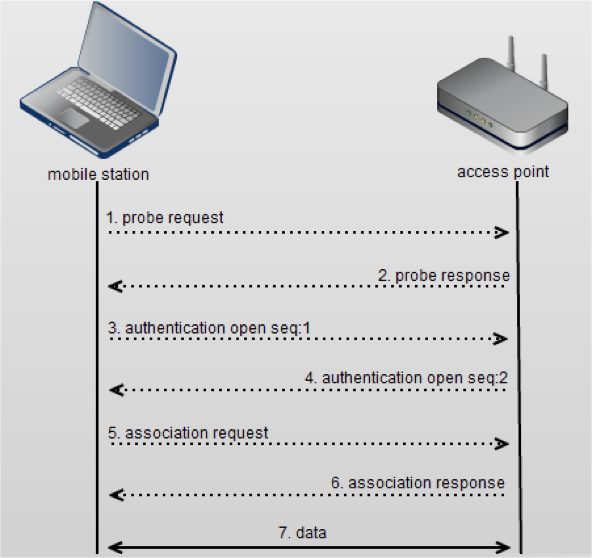
\includegraphics[width=0.8\textwidth]{probe.png}
    \caption{Wi-Fi connection establishment}
    \label{fig:probe}
\end{figure}

\section{Location detection}
There are exist couple of techniques which allows to determine location of certain device that supports Wi-Fi. This techniques mostly based on trilateration algorithm. According to paper by Edwin George Vaapparamban \cite{edwin16} Probe requests are signals that are continuously broadcast from devices with WiFi technology, such as smartphones, laptops, and tablets. When a WiFi client wants to get connected to a WiFi network, the first method is scanning for beacon frames, which are frames broadcast by WiFi routers to tell about their presence to WiFi clients. The second method is sending probe requests, which also contains the unique MAC address of the device, as well its type, brand, manufacturer, and model. Since a WiFi client itself can initiate a connection to a WiFi router instead of waiting for a beacon frame from the router, use of probe requests is preferable. The probe requests are not encrypted, and can be captured and decoded with the help of wireless sniffers passively, without connecting to a particular network or transmitting any signal.

\subsection{Our solution}
The naive solution that we supposed to do is to sniff all packets that are going inside our access point coverage. Sniffing all packets have one big advantage that we can handle every active device. Hotspot 2.0 is an initiative of the Wi-Fi Alliance to stream- line network discovery and selection, aiming to create a roaming experience matching that of cellular phones. It allows clients to discover hotspots for which they have appropriate credentials, and provides automatic roaming between wireless networks. Hotspot 2.0 relies on 802.11u, a standard providing a communication channel even when the station is unassociated with an Access Point (AP). Stations use this channel to query an AP for network access information using the Access Network Query Protocol (ANQP). For example, ANQP can be used for discovering which credentials can be used to authenticate to a hotspot. Using this solution we had issues with setuping access point signal strength, but this solution gave us implausible results. Because of huge amount of devices inside our building we got a lot of noise and our access point had problems to determine signal strength.

We suppose that restricted area is located inside the building. In this case we can assume that inside building walls can decrease strength of Wi-Fi signal. When someone with Wi-Fi device walks inside building, every time he changes room, his device sends probe requests to find the best available network connection. In our particular experiment new probe requests are sent every time someone with a device enters the room. This allows us to continue our research using only the probe requests sniffing technique. According to Mathy Vanhoef the probe requests include data in their frame body under the form of Information Elements (IEs), also called tagged parameters, or tags. These IEs are not mandatory and are used to advertise the support of various functionalities. They are generally composed of several subfields whose size can range from one bit to several bytes. 

\section{Proof-of-concept}
To implement prototype we used notebook with Wi-Fi module running on Ubuntu 16.04. To be able to sniff packets we turned on monitor mode on Wi-Fi module via \textbf{airmon-ng} utility.

\begin{bashcode}
airmon-ng start wlan0
airmon-ng check kill 
\end{bashcode}

Core module is written on python using library scapy. Script below sniffs all packets in coverage area, checks sender/receiver mac address with blacklist and if it found any matches, sends request to notification server (telegram bot). Blacklist updates from server every 30 seconds.

\begin{figure}[h]
    \centering
    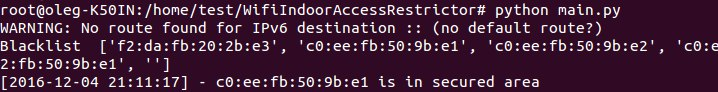
\includegraphics[width=0.8\textwidth]{console}
    \caption{Output of console application}
    \label{fig:console}
\end{figure}

\begin{pythoncode*}{label="main.py"}
#!/usr/bin/env python
# -*- coding: utf-8 -*-


from time import gmtime, strftime
from scapy.all import *
import os
import time
import thread
import urllib3
http = urllib3.PoolManager()

from threading import Timer,Thread,Event

class perpetualTimer():

   def __init__(self,t,hFunction):
      self.t=t
      self.hFunction = hFunction
      self.thread = Timer(self.t,self.handle_function)
      self.thread.daemon = True

   def handle_function(self):
      self.hFunction()
      self.thread = Timer(self.t,self.handle_function)
      self.thread.start()

   def start(self):
      self.thread.start()

   def cancel(self):
      self.thread.cancel()







## blacklist = open("black.txt","r".read().split("\n")
logfile = open("logs.txt","a+")
breaks=[]
blacklist=[]


def getBlackList():
    return http.request("GET", "http://dagmeet.appspot.com/LIST").data.split("\n")

def updateBlackList():
    global blacklist
    print blacklist
    newbl = getBlackList()
    if blacklist != newbl:
        blacklist = newbl
        print "Blacklist updated: ",blacklist

def request(str):
    http.request("GET", "http://dagmeet.appspot.com/NOTIFY", fields={"mac": str})
    

def notify(addr):
    if addr not in breaks:
        time = strftime("%Y-%m-%d %H:%M:%S", gmtime())
        logfile.write("[{0}] - {1} is in secured area\n".format(time, addr))
        print "[{0}] - {1} is in secured area".format(time, addr)
        request("[{0}] - {1} is in secured area".format(time, addr))
        breaks.append(addr)

def PacketHandler(pkt):
    if pkt.addr2 in blacklist:
        notify(pkt.addr2)
    elif pkt.addr1 in blacklist:
        notify(pkt.addr1)

blacklist = getBlackList()
print "Blacklist ", blacklist

t = perpetualTimer(30,updateBlackList)
t.start()
sniff(iface="mon0", prn = PacketHandler)
\end{pythoncode*}

The managment and notification part is written on python using flask and telegram-bot modules. User has only one command to get administrative access /admin <password>. Administrators have multiple commands for adding mac to blacklist, removing from it, geting full list of banned devices. Also administrators get notifications about access control breach via that telegram bot.

\begin{figure}[h]
    \centering
    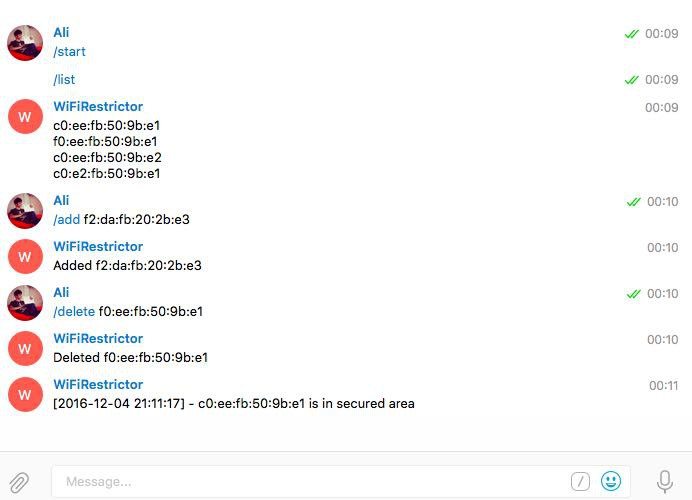
\includegraphics[width=0.8\textwidth]{bot}
    \caption{Telegram bot}
    \label{fig:bot}
\end{figure}

\begin{pythoncode*}{label="bot\_main.py"}
#!/usr/bin/env python 
# -*- coding: utf-8 -*- 
from __future__ import unicode_literals 

import site 
import os.path 
import logging 
import json
import hashlib
site.addsitedir(os.path.join(os.path.dirname(__file__), 'libs')) 

import telegram 
from flask import Flask, request 

from google.appengine.ext import db




app = Flask(__name__) 

 
TOKEN = ''
URL = 'dagmeet.appspot.com' 
password = "" # Very strong password's hash
global bot 
bot = telegram.Bot(token=TOKEN) 
admins = []

def checkPassword(str):
    h = hashlib.sha256()
    h.update(str)
    return h.hexdigest() == password

class Record(db.Model):
    address = db.StringProperty()


@app.route('/LIST', methods=['GET']) 
def getList():
    records = db.GqlQuery("SELECT * FROM Record")
    response = ""
    for record in records:
        response+=record.address
        response+="\n"
    return response

def addRecord(str):
    str = str.replace("-","")
    str = str.replace("'","")
    record = Record(address=str)
    record.put()

def deleteRecord(str):
    str = str.replace("-","")
    str = str.replace("'","")
    records = db.GqlQuery("SELECT * FROM Record WHERE address=:1",str)
    for record in records:
        record.delete()




@app.route('/NOTIFY', methods=['GET']) 
def notify():
    for admin in admins:
        bot.sendMessage(chat_id=admin, text=request.args.get("mac"))

@app.route('/HOOK', methods=['POST']) 
def webhook_handler(): 
    if request.method == "POST": 
        update = telegram.Update.de_json(request.get_json(force=True))
        try:
            chat_id = update.message.chat.id 
            text = update.message.text
            text = text.lower()
            if text.startswith("/admin"):
                data = text.split(" ")
                if checkPassword(data[1]):
                    admins.append(chat_id)
                    bot.sendMessage(chat_id=chat_id, text="Access granted")
                else:
                    bot.sendMessage(chat_id=chat_id, text="Access denied")
            if text.startswith("/add") and chat_id in admins:
                data = text.split(" ")
                if len(data)==2:
                    addRecord(data[1])
                    bot.sendMessage(chat_id=chat_id, text="Added "+data[1])
                else:
                    bot.sendMessage(chat_id=chat_id, text="Syntax error; /add <mac_addr>")
            if text.startswith("/delete") and chat_id in admins:
                data = text.split(" ")
                if len(data)==2:
                    deleteRecord(data[1])
                    bot.sendMessage(chat_id=chat_id, text="Deleted "+data[1])
                else:
                    bot.sendMessage(chat_id=chat_id, text="Syntax error; /delete <mac_addr>")
            if text.startswith("/list") and chat_id in admins:
                bot.sendMessage(chat_id=chat_id, text=getList())
            logging.getLogger().setLevel(logging.INFO) 
            logging.info('===============TEXT=================' + text) 
        except AttributeError:
            print "a"
    return 'ok' 

 
@app.route('/set_webhook', methods=['GET', 'POST']) 
def set_webhook(): 
    s = bot.setWebhook('https://%s/HOOK' % URL) 
    if s: 
        return "webhook setup ok" 
    else: 
        return "webhook setup failed" 

@app.route('/') 
def index(): 
    return '.' 
\end{pythoncode*}

\section{Conclusion}
We achieved our main goal to detect violation of restricted areas inside buildings. Our solution is not perfect and we have to do a lot of work because Wi-Fi based location detection is a very complicated topic. But at this point we have working application which is easy to use. The main problems is to reduce the noise and determine position more accurate.


\begin{thebibliography}{9}

\bibitem{edwin16}
  Edwin George Vaapparamban,
  \emph{People Counting and occupancy Monitoring using WiFi Probe Requests and Unmanned Aerial Vehicles},
  FIU Digital Commons, Florida,
  2016.
\bibitem{mathy16}
  Mathy Vanhoef, et. all,
  \emph{Why MAC Address Randomization is not Enough: An Analysis of Wi-Fi Network Discovery Mechanisms},
  University of Leuven, Leuven,
  2016.

\end{thebibliography}

\end{document}